\section{Introduction}
A long-term goal of robotics research is the introduction of intelligent household robots.
To be effective, such robots will need to perform complex tasks (e.g., setting a dinner table, doing laundry)
over long horizons. Planning for these long-horizon tasks is infeasible
for state-of-the-art motion planners, making the need
for a hierarchical system of reasoning apparent.

One way to approach hierarchical planning is through combined \emph{task and motion planning} (TAMP). In this
approach, an agent is given a symbolic, logical characterization of actions (e.g., move, grasp,
putdown), along with a geometric encoding of the environment. The hierarchical separation of high-level, symbolic task planning
from low-level, geometric motion planning enforces abstraction:
the task planner maintains no knowledge of the environment geometry, and the
motion planner has no understanding of the overall goal.
Efficient integration of these two types of reasoning is challenging, and recent research has
proposed several methods for it~\cite{srivastava2014combined, kaelbling2011hierarchical,
lagriffoul2014orientation, GarrettWAFR14, dornhege2012semantic}.

\begin{figure}[t]
  \centering
    \noindent
    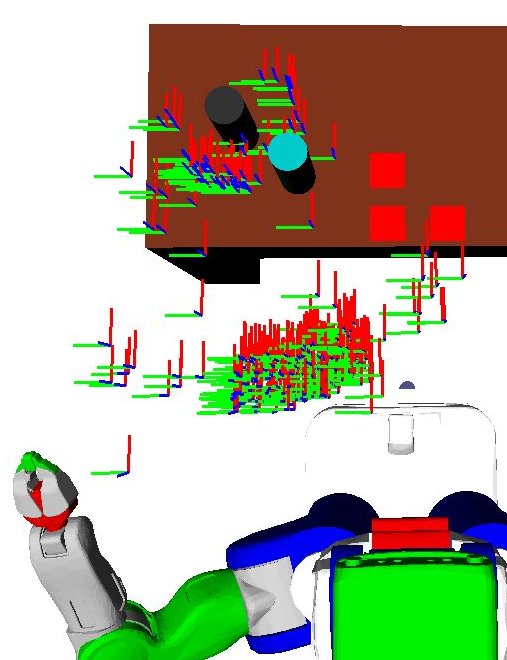
\includegraphics[scale=0.2]{images/move_grasp.png}\hspace{10 mm}
    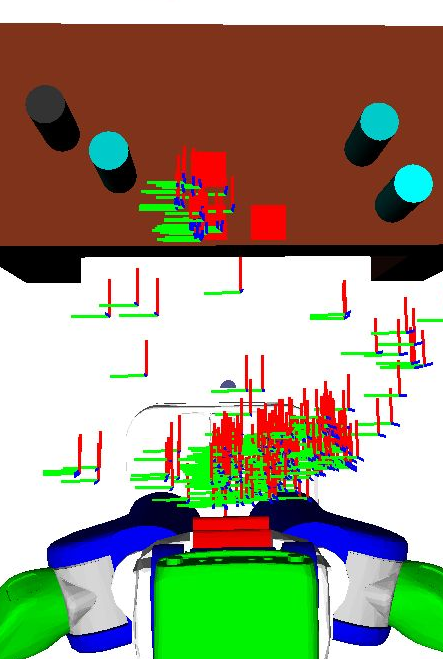
\includegraphics[scale=0.2]{images/move_putdown.png}
  \caption{Screenshots showing some distributions learned by our system in a simulated pick-and-place
    domain. We use reinforcement learning to train good sampling distributions for continuous motion
    planning parameters in long-horizon tasks. The robot is tasked with grasping the black cylinder and putting it down on the
    central red square. The left image shows learned base motion (blue) and grasping (green) distributions,
    and the right shows learned base motion (blue) and putdown (green) distributions. The grasping policy
    learned automatically to avoid the region close to the light blue obstruction. These distributions are
    optimized to reduce the number of motion planner calls needed to produce a complete plan.}
  \label{fig:cover}
\end{figure}

Our methods build on the TAMP system presented by Srivastava et al.~\cite{srivastava2014combined}.
In this system, a (classical) task planner produces a symbolic plan containing
a sequence of actions to reach a goal state. Then, in a process known as \emph{plan refinement},
candidate values are proposed for the continuous variables in this symbolic plan.
These values are checked locally for feasibility by calling a motion planner.
Both the task planner and the motion planner are used as black boxes.

The authors propose an \emph{interface layer} for refining the plan into a set
of collision-free trajectories; it performs an exhaustive backtracking search over a
set of sampled candidate parameter values. If a motion planning feasible
refinement is not found within the resource limit, symbolic error information is
propagated back to the task planner, and a new symbolic plan is produced.

The system, however, relies on hand-coded discretizations to sample continuous values for these
plan parameters. Designing these heuristic sampling distributions requires substantial effort,
as they are tuned based on geometric attributes of the environment and its objects, meaning they
must be recalibrated when running the system in a new setting. Further,
the discretizations must be fairly coarse to allow reasonable search speeds, meaning they inherently lack
robustness to increased environmental complexity. In this paper, we present a reinforcement
learning method to train good continuous proposal distributions for sampling plan parameter values.

Unpublished work that is currently in progress extends this system to achieve completeness by
maintaining a \emph{plan refinement graph}, whose nodes each store a valid
symbolic plan (that reaches the goal) and its current parameter values. This makes it possible to interleave
partial refinement of several plans. In this paper, we also develop a method for making the meta-level decision of
\emph{which} plan to try refining next.

Other TAMP paradigms use similar hand-coded heuristics to sample continuous values for symbolic variables.
While our method is specific to this architecture, it can be adapted for these systems.

Reinforcement learning (RL) refers to the process of an agent learning a policy (a mapping from states to actions)
in its environment that maximizes rewards. Zhang and Dietterich~\cite{JobShopSched} first applied the RL framework
to planning problems, using a job shop scheduling setting. In this work, we take inspiration from
their approach; we apply RL to plan refinement in a TAMP system. We implement our approach using methods adapted from
Zucker et al.~\cite{workspacebias}, who train a configuration space sampler for motion planning
using features of the discretized workspace.

The four contributions of our work are as follows: 1) we present randomized refinement, a local search
algorithm for plan refinement that is easily formulable as an MDP; 2) we formulate plan refinement in the
RL framework and learn a policy for this MDP; 3) we train heuristics to search intelligently
through a plan refinement graph, allowing us to decide \emph{which} plan to try refining next;
and 4) we present experiments to evaluate our approach in a variety of simulated
domains. Our results demonstrate that our approach yields significantly improved
performance over that of hand-coded discretization of the plan refinement sample space.
